%% fundamentals.tex
%%

%------------------------------------------------------------------------------------------------
\section{Grundlagen}
\label{sec:Grundlagen}
%------------------------------------------------------------------------------------------------

Gemäß der einleitenden Motivation aus Sektion \ref{sec:Einleitung} wird nun mit der Erläuterung der Begrifflichkeiten für die spätere Zuordnung der einzelnen Komponenten aus dem Bereich \ac{iot} begonnen. Dies umfasst hierbei die Definition eines smarten Gerätes mit einer Darstellung der Architektur eines solchen Systems. 
Anschließend folgt ein Überblick über die derzeit geltenden gesetzlichen Kontexte, die bezüglich der Einhaltung von Datenschutz eine Bewertung erlauben. Darauf aufbauend werden anhand der gewählten gesetzlichen Rahmenwerke, die im Falle dieser Ausarbeitung die \ac{dsgvo} und \ac{ftc} umfassen, Beispiele für deren Definition unterschiedlicher Datenklassen vorgestellt und Vergleiche im Umfang und der Präzision der entsprechenden Definitionen vorgenommen. 
In Bezug auf die Erhebung personenbezogener Daten erfolgt eine Einordnung möglicher Gefahren für den einzelnen Nutzer, die durch nicht-datenschutzkonformes Verarbeiten der Daten durch die Geräte entstehen können. 
Abschließend werden die beiden untersuchten Bereiche des Smart Home und der Smart City in einer globalen Betrachtung smarter Umgebungen entsprechend kategorisiert.\\

%%------------------------------------------------------------------------------------------------
\subsection{Geräte des \acl{iot}}
\label{sec:Grundlagen:ssec:Geräte des Internet of Things}
%%------------------------------------------------------------------------------------------------

Im Rahmen der aktuellen Definitionen von Geräten des \ac{iot}, oder auch Smart Devices genannt, werden diese als Klasse von Geräten beschrieben, die unter Verwendung von Sensoren Informationen aus ihrer Umwelt aufnehmen und auf Basis dieser Daten gezielt Instruktionen durchführen. Hierbei reicht die Bandbreite von Gadgets des alltäglichen Gebrauchs, u.a. Mobiltelefone oder Smart Watches, bis hin zu autonomen Robotern aus der Industrie 4.0, die über Kameras und hochempfindliche Messgeräte mit ihrer Umwelt in Wechselwirkung treten \cite{Li2015}. 
Dies geschieht hierbei ohne jegliches Zutun eines Menschen über das Internet oder ein internes Netzwerk. Architektonisch lässt sich das \ac{iot} in drei Schichten unterteilen. Diese können basierend auf der Definition von \cite{Seliem2018} folgendermaßen darstellen:

\begin{itemize}
    \item Die \textbf{Geräte-Schicht} (Device Layer) beschreibt hierbei die Schicht mit allen physikalischen Ressourcen, die Daten sammeln und regulieren. Diese Schicht beinhaltet somit die Grundgesamtheit aller heterogenen und ressourcen-beschränkten Geräte.
    \item Die \textbf{Plattform-Schicht} (Platform Layer) repräsentiert die klassischen \\Netzwerk-Schicht (Network Layer) im OSI Modell. Diese Schicht integriert die notwendige Vorverarbeitung der Daten und reduziert somit die Anforderungen an die Ressourcen innerhalb der Applikation-Schicht.
    \item Die \textbf{Applikation-Schicht} (Application Layer) setzt sich wiederum aus zwei Teilen zusammen. Auf der einen Seite die Unterstützungsschicht (Support Layer), auf der das Edge Computing und die analytischen Dienste betrieben werden und auf der anderen Seite die Applikation-Dienst-Schicht (Application Service Layer), die die notwendige Unterstützung bezüglich der Rechenressourcen für die \ac{iot} Infrastruktur bereitstellt.
\end{itemize}

\begin{figure}
    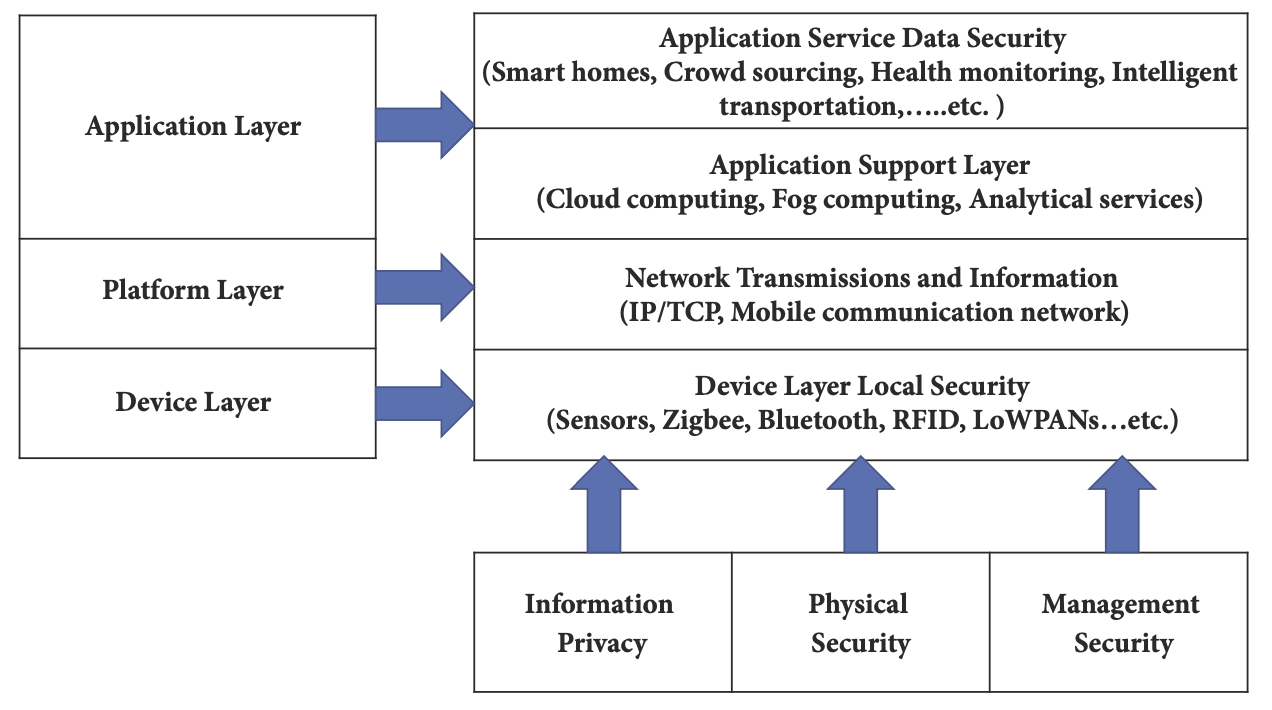
\includegraphics[width=\textwidth]{fundamentals/pictures/IoT_Layer_Architecture}
    \caption{Drei Schichten Architektur des \ac{iot} zur Untergliederung der einzelnen Komponenten gemäß \cite{Seliem2018}}
    \label{fig:drei-schichten-iot}
\end{figure}

\noindent Wie bereits in der Illustration \ref{fig:drei-schichten-iot} angedeutet, lassen die einzelnen Schichten eine feinere Unterteilung im Rahmen unterschiedlichster Nutzungsfälle zu. Beispielsweise werden in anderen Publikationen, diese Thematik betreffend, auch vier Schichten für eine genauere Unterteilung der einzelnen Bestandteile genutzt. Da dies als Teil dieser Ausarbeitung jedoch nicht relevant ist, werden auch im späteren Verlauf nur die Drei-Schicht-Modelle verwendet.

%------------------------------------------------------------------------------------------------
\subsection{Rechtliche Rahmenbedingungen}
\label{sec:Grundlagen:ssec:Rechtliche Rahmenbedingungen}
%------------------------------------------------------------------------------------------------

Zur grundlegenden Bewertung und Einordnung der erhobenen Datenklassen besteht die Möglichkeit je nach Rechtssystem unterschiedliche Regularien anzu-wenden. Die beiden wichtigsten Vertreter ihrer Art sind einerseits die \acl{gdpr} beziehungsweise \acl{dsgvo} innerhalb des europäischen Rechtssystems und die \acl{ftc} als staatliche Institution, die die Interessen der US-Bürger in unterschiedlichen Ressorts bedient. 
Für beide Vertreter gilt, dass sie den Umgang mit \ac{pii}, \ac{nonpii} und personenbezogenen Daten beschreiben und somit sicherstellen, dass bestimmte Standards an Sicherheit und Privatsphäre umgesetzt werden. Die genaue Abgrenzung hinsichtlich der Unterschiede zwischen den beiden gewählten Vertretern wird nachfolgend nochmals genauer erläutert.

%------------------------------------------------------------------------------------------------
\subsubsection{\acl{gdpr}}
\label{sec:Grundlagen:ssec:Rechtliche Rahmenbedingungen:sssec:GDPR}
%------------------------------------------------------------------------------------------------

Durch Inkrafttreten der \\ \ac{gdpr} / \ac{dsgvo} am 25.05.2018 wurde von der \acl{eu} ein einheitlicher Katalog an Regeln geschaffen, der den allgemeinen Umgang bezüglich der Erhebung und der Verarbeitung von Daten im europäischen Raum beschreibt. 
Ziel sind hierbei (globale) Unternehmen und Einrichtungen, die innerhalb der \acl{eu} als Teil ihrer Dienstleistungen Daten von \acs{eu}-Bürgern erheben und diese verarbeiten. Als Nachfolger der \textbf{\textit{Data Protection Directive 95/46/EC}} löste sie diese mit der erstmaligen Einführung der \ac{gdpr} 2016/679 am 24.05.2016 ab. 
Zweck dieses Rahmenwerkes war die Harmonisierung der Datenschutz- und Privatsphäre-Regelungen innerhalb der \acl{eu} \cite{Bastos2019}.

\noindent Neben der Definition von zentralen Begrifflichkeiten und Eckpunkten stehen die Formulierung von Prinzipien im Mittelpunkt des Gesetzestextes. Zur Einordnung dieser, wird beginnend mit der nachfolgenden Auflistung ein Überblick über die beteiligten rechtlichen Entitäten auf Basis von \cite{DSGVOArt4} gegeben.

\begin{itemize}
    \item \textbf{\acl{ds}} / \textbf{betroffene Person} beschreibt eine natürliche Person im Kontext des jeweiligen Rechtsstaates.
    \item \textbf{\acl{dc}} / \textbf{Verantwortlicher} beschreibt eine natürliche oder rechtliche Person, die den Zweck und den Vorgang der Verarbeitung der persönlichen Daten definiert.
    \item \textbf{\acl{dp}} / \textbf{Auftragsverarbeiter} beschreibt eine natürliche oder rechtliche Person, die auf Anordnung des \textbf{Verantwortlichen} die persönlichen Daten verarbeitet.
\end{itemize}

\noindent Im späteren Verlauf dieser Arbeit werden für das bessere Verständnis nur noch die Abkürzungen der englischen Bezeichnungen für die Akteure verwendet. Darauf aufbauend stehen die Grundprinzipien der \ac{dsgvo} als Wegweiser für die Rechte dieser "Personen". 
Nachfolgend aufgelistet stehen die \textbf{sieben} Grundprinzipien, die im Rahmen der Datenverarbeitung durch \textbf{Verantwortliche} und \textbf{Auftragsverarbeiter} einzuhalten sind. Die Formulierungen sind anhand von \cite{DSGVOArt5} präzisiert worden:

\begin{itemize}
    \item \textbf{Fair, lawful and transparent processing} / \textbf{Rechtmäßigkeit, Verarbeitung nach Treu und Glauben, Transparenz} \\ Die Verarbeitung von personenbezogenen Daten muss für die betroffene Person nachvollziehbar sein.
    \item \textbf{Purpose Limitation} / \textbf{Zweckbindung} \\ Die Verarbeitung der personenbezogenen Daten darf nur im Rahmen des Zwecks der Erhebung geschehen.
    \item \textbf{Data Minimisation} / \textbf{Datenminimierung} \\ Die Datenmenge muss dem Zweck angemessen und somit nur auf das not-wendige Maß für die Verarbeitung beschränkt sein.
    \item \textbf{Accuracy} / \textbf{Richtigkeit} \\ Die Daten müssen in korrekter Form vorliegen und auf dem aktuellen Stand gehalten werden. Alle nicht korrekten Einträge müssen gelöscht werden.
    \item \textbf{Storage Limitation} / \textbf{Speicherbegrenzung} \\ Die Daten dürfen nur so lange gespeichert werden, wie es dem Zweck der Verarbeitung dient.
    \item \textbf{Integrity and Confidentiality} / \textbf{Integrität und Vertraulichkeit} \\ Die Verarbeitung der Daten muss so gestaltet werden, dass ein bestimmtes Maß an Sicherheit gewährleistet werden kann, um unbefugten Zugriff oder Verlust zu vermeiden.
    \item \textbf{Accountability} / \textbf{Rechenschaftspflicht} \\ Der \textbf{\ac{dc}} ist für die Einhaltung der obigen \textbf{sechs} Prinzipien verantwortlich und muss dies nachweisen können.
\end{itemize}

%------------------------------------------------------------------------------------------------
\subsubsection{\acs{etsi} EN 303 645}
\label{sec:Grundlagen:ssec:Rechtliche Rahmenbedingungen:sssec:ETSI EN 303 645}
%------------------------------------------------------------------------------------------------

Die im Rahmen der \ac{dsgvo} definierten Richtlinien für den Datenschutz der europäischen Bürger und Institutionen sind jedoch nicht auf die Entwicklung von sicheren \ac{iot}-Systemen anwendbar. Aus diesem Grund wurde von der europäischen Normungsorganisation \acl{etsi} der ETSI EN 303 645 als europäischer Standard, definiert, der die Basisanforderungen an die IT-Sicherheit von vernetzten Geräten für Verbraucherinnen und Verbraucher, beispielsweise im Smart Home, spezifiziert. 
Hiermit werden Empfehlungen für die sichere Entwicklung (\acl{sbd}) von \ac{iot}-Geräten und deren Anwendungen erhoben \cite{BSI2020}. In Kombination mit der im August 2021 veröffentlichten Prüfspezifikation ETSI TS 103 701 erlaubt dieser Standard die Prüfung von Geräten des Smart Home Bereichs und die Erteilung von IT-Sicherheitskennzeichen an die verschiedenen Produktkategorien \cite{BSI2022}.

%------------------------------------------------------------------------------------------------
\subsubsection{\acl{ftc}}
\label{sec:Grundlagen:ssec:Rechtliche Rahmenbedingungen:sssec:FTC}
%------------------------------------------------------------------------------------------------

Die \acl{ftc}, auch Bundeshandelskommission genannt, stellt eine politische Institution im amerikanischen Raum dar, der die Regulation der Datensicherheit und Privatsphäre obliegt. Neben dem Ressorts des Datenschutzes deckt sie auch allgemein den Verbraucherschutz der amerikanischen Bürger ab. 
Hierunter fällt unter anderem die Kontrolle von unlauterem Wettbewerb oder rechtswidrigen Geschäftsmethodiken. Weitere Beispiele des Service-Portfolios sind die Beratung von Endkunden bezüglich Einkauf, Krediten und Identitätsdiebstahl bis hin zu Thematiken des wirt-schaftlichen Kontexts. 
Somit beschreibt die \ac{ftc} nicht nur die Regeln, sondern kann diese auch effektiv umsetzen \cite{FTC}. Als gleichwertiges Organ kann hier die \textbf{\textit{Abteilung für Recht der Europäischen Kommission}} gesehen werden \cite{FTCEU}. Bezüglich des Datenschutzes gilt es jedoch zu beachten, dass innerhalb des amerikanischen Rechtssystems kein zentrales Organ über alle Bundesstaaten hinweg definiert ist, das die Einhaltung dieser Regeln kontrolliert. 
Allgemein gilt, dass jedes amerikanische Unternehmen ihre Ansprüche an den Datenschutz und die Privatsphäre selbst definiert und deren Einhaltung entsprechend umsetzt. Kommt das Unternehmen diesen selbsterlegten Anforderungen nicht nach, ist vorerst mit keinen Disziplinarmaßnahmen von Seiten des Staates zu rechnen, sondern es wird im Wettbewerb nur als nicht vertrauenswürdiger Geschäftspartner behandelt \cite{DatenschutzOrg2022}.

%------------------------------------------------------------------------------------------------
\subsection{Klassifikation von Daten}
\label{sec:Grundlagen:ssec:Klassifikation von Daten}
%------------------------------------------------------------------------------------------------

Im Kontext der nun eingeführten Grundlagen für die Rechtssprechung bezüglich des Datenschutzes im europäischen und angloamerikanischen Raum, werden nachfolgend die unterschiedlichen Klassen von Daten eingeführt, die in den jeweiligen Systemen existieren. 
Der Schwerpunkt der Auflistung liegt hierbei auf den Daten, die im Allgemeinen von Personen gesammelt, beziehungsweise erhoben werden und betrachtet beispielsweise keine Kontroll-Daten beziehungsweise Lebenszyklus-Daten aus technischen Systemen. 
Wie bereits in \fullref{sec:Einleitung} erwähnt, können die gesammelten Daten auf Basis ihres Informationsgehaltes in unterschiedliche Kategorien eingeteilt werden. Neben der Einteilung in \ac{pii} und \ac{nonpii} wird des Weiteren in personenbezogene, nicht personenbezogene, anonymisierte und pseudonymisierte Daten unterschieden.

\paragraph{\acf{pii}.}
\label{sec:Grundlagen:para:Personal Identifiable Information}
Der Begriff der \ac{pii} stammt ursprünglich aus dem amerikanischen Raum und wird innerhalb unterschiedlichster Institutionen der USA verwendet. Jedoch gilt es hier zu beachten, dass trotz desselben Rechtssystems keine einheitliche Definition existiert und somit die gewählten Beschreibungen nicht rechtlich fundiert sind. 
Basierend auf der Handreichung der \ac{nist}, die extreme Ähnlichkeiten bezüglich der Definition von \ac{ftc} aufweist, handelt es sich bei \acs{pii} um Informationen, die es ermöglichen Rückschlüsse auf die Person zu ziehen, von der die Daten stammen \cite{Matuszewska2021,NIST2010}. Des Weiteren findet eine weitere Unterteilung in sogenannte \textbf{verknüpfbare Informationen} und \textbf{verknüpfte Informationen} statt. Nachfolgend werden je Kategorie Beispiele aufgeführt:

\begin{itemize}
	\item \textbf{verknüpfte Informationen}:
		\begin{itemize}
			\item (vollständiger) Name
			\item E-Mail Adresse
			\item Cookies
			\item Geräte-ID
		\end{itemize}
	\item \textbf{verknüpfbare Informationen}:
		\begin{itemize}
			\item Vorname oder Nachname
			\item Land, Bundesland, Stadt, PLZ
			\item Geschlecht
			\item Rasse
		\end{itemize}
\end{itemize}

\noindent Im Vergleich zu persönlichen Daten im Sinne der \ac{dsgvo} umfassen die \acs{pii} deutlich weniger Daten, die in diese Kategorie fallen.

\paragraph{\acf{nonpii}.}
\label{sec:Grundlagen:para:Non Personal Identifiable Information}
Im Kontrast zu den \ac{pii} stellen die \ac{nonpii} eine Klasse an Daten dar, deren alleinstehende Verwendung kein Tracking oder eine Identifikation eines Individuums erlaubt. Beispielsweise gehören für manche AdTech-Unternehmen die Informationen wie zum Beispiel Geräte-ID oder Cookies, im Gegensatz zu den bereits definierten \textbf{verknüpften Daten}, aus \ac{pii} zu den \ac{nonpii}. Diese Abweichungen sind aufgrund der beschriebenen Problematik hinsichtlich der fehlenden rechtlichen Fundamente im amerikanischen Gesetzeskontext durchaus üblich und müssen somit für jeden Einzelfall geprüft werden. Zur Kategorie von \ac{nonpii} gehören nach \cite{Matuszewska2021} unter anderem:

\begin{itemize}
	\item Aggregierte Statisktiken zur Nutzung von Produkten
	\item Teilweise oder vollständig maskierte IP-Adressen
\end{itemize} 

\paragraph{Personenbezogene Daten.}
\label{sec:Grundlagen:para:Personenbezogene Daten}
Personenbezogene Daten "[beschreiben] alle Informationen, die sich auf eine identifizierte oder identifizierbare natürliche Person [...] beziehen" \cite{DSGVOArt4}. Somit gehören dementsprechend auch Cookies, Geräte-IDs und IP-Adressen zu den schützenswerten Informationen, womit sich die \ac{dsgvo} deutlich von ihrem amerikanischen Äquivalent unterscheidet. Weitere Beispiele für personenbezogene Daten sind nach \cite{Matuszewska2021} oder \cite{DSGVOPerDa}:

\begin{itemize}
	\item Standortdaten
	\item Werbekennung des Handys
	\item Genetische Daten
	\item Biometrische Daten
	\item Gesundheitsdaten
\end{itemize}

\noindent Entsprechend der Granularität und Präzision der Formulierungen in der \ac{dsgvo} kann durchaus von einer strikteren Fassung im Vergleich mit dem amerikanischen Regelwerkes ausgegangen werden. Dies findet sich beispielsweise auch bei der Verhängung von Strafen bezüglich nicht konformen Handelns innerhalb der einzelnen Gesetzeskontexte wieder.

%%------------------------------------------------------------------------------------------------
%\subsubsection{Anonymisierte Daten}
%\label{sec:Grundlagen:ssec:Klassifikation von Daten:sssec:Anonymisierte Daten}
%%------------------------------------------------------------------------------------------------

\paragraph{Anonymisierte Daten.}
\label{sec:Grundlagen:para:Anonymisierte Daten}
Bei anonymisierten Daten handelt es sich um \textbf{nicht personenbezogene Daten}. Unter Verwendung dieser Art von Informationen kann keinerlei Person identifiziert oder mit den Daten in Verbindung gebracht werden. Aus diesem Grund wird die Handhabung von anonymen Daten von der \ac{dsgvo} auch nicht weiter reguliert. Dies ist zum Beispiel mittels des Erwägungsgrundes 26 \cite{DSGVOEg26} innerhalb der \ac{dsgvo} geregelt. Beispiele für anonymisierte Daten sind somit den Referenzen aus \ac{nonpii} gleichzusetzen.

%%------------------------------------------------------------------------------------------------
%\subsubsection{Pseudonymisierte Daten}
%\label{sec:Grundlagen:ssec:Klassifikation von Daten:sssec:Pseudonymisierte Daten}
%%------------------------------------------------------------------------------------------------

\paragraph{Pseudonymisierte Daten.}
\label{sec:Grundlagen:para:Pseudonymisierte Daten}
Mittels der Pseudonymisierung von Daten ist es für den Betrachter dieser Daten nicht mehr möglich, ohne die Verwendung von zusätzlichen Informationen einen Bezug zu einem spezifischen Individuum herzustellen \cite{DSGVOArt4}. 
Somit wird es möglich auch höchst sensible Daten durch eine Pseudonymisierung für die Verwendung in einem anderen Kontext freizugeben. Eine mögliche Anwendung ist zum Beispiel das gezielte Ersetzen von Informationsbestandteilen (personenbezogene Daten) durch berechnete Einträge oder Codes, die später eine erneute Substitution ermöglichen.

%------------------------------------------------------------------------------------------------
\subsection{Gefahren für die Privatsphäre.}
\label{sec:Grundlagen:ssec:Gefahren für die Privatsphäre}
%------------------------------------------------------------------------------------------------

Anhand der vorgestellten Datenkategorien in \ref{sec:Grundlagen:ssec:Klassifikation von Daten} werden nun die möglichen Gefahren für die Nutzer von \ac{iot}-Geräten aufgezeigt und deren Auswirkungen, die im Rahmen der nachfolgenden Analyse für Geräte des Smart Home und Smart City Kontextes eine wichtige Rolle spielen. Entsprechend der Verwendung in mehreren englischsprachen Arbeiten, werden auch hier die Gefahren in internationaler Notation aufgeführt. 
Die nachfolgend aufgeführte Liste erhebt hierbei in keinster Weise einen Anspruch auf Vollständigkeit und kann in unterschiedlichen Kontexten in Bezug auf den Untersuchungsgegenstand beliebig erweitert werden.

\paragraph{(User) Identification.}
\label{sec:Grundlagen:para:User Identification}
Die (User) Identification beschreibt die Möglichkeit zur Charakterisierung einer Person (oder einer Entität) anhand von personenbezogenen Daten (z.B. Name, Adresse oder Standort) und einer anschließenden Veröffentlichung deren Identität. Daraus resultierende Gefahren sind neben der Verletzung der Privatsphäre des Individuums zusätzlich das Ermöglichen weiterer Eingriffe in Form der nachfolgenden Gefahren für den Nutzer. Dies könnte zum Beispiel das gezielte Sammeln von Informationen sein, die wiederum mit dem Nutzer in Verbindung gebracht werden können und somit eine gezieltes Profiling des Nutzers ermöglicht \cite{Seliem2018}.

\paragraph{(User) Tracking.}
\label{sec:Grundlagen:para:User Tracking}
Aufbauend auf dem vorherigen Eingriff in die Privatsphäre und den Datenschutz des Nutzers, besteht die Gefahr eines (User) Trackings. Hierbei werden die gesammelten Daten über einen bestimmten Nutzer, meist in Form von Standortdaten, dazu verwendet dessen Aufenthaltsorte zu lokalisieren. Hiermit ergeben sich für die unterschiedlichen Dienstbetreiber die Möglichkeit unter Verwendung von beispielsweise Machine Learning Algorithmen das Verhalten bestimmter Ziele zu erlernen und somit auf Basis seines Standorts entsprechende Angebote zu unterbreiten \cite{Seliem2018}.

\paragraph{Monitoring.}
\label{sec:Grundlagen:para:Monitoring}
Diese Gefahr bezieht sich direkt auf das Erheben von Nutzungsdaten eines Gerätes im Kontext von Rekonstruktion vergangener Interaktion des Nutzers mit dem Gerät. Basierend auf diesen Informationen lassen sich beispielsweise Muster aus dem Alltag des Nutzers identifizieren, die wiederum in anderer Art und Weise wiederverwendet werden können \cite{Seliem2018}.

\paragraph{Profiling.}
\label{sec:Grundlagen:para:Profiling}
Die Methodik des Profilings erstellt auf Basis aggregierten Datenmaterials ein Profil eines Individuums, welches dazu verwendet werden kann, eine genauere Beschreibung davon zu erstellen, welche Interessen und Bedürfnisse eine Person verfolgt. Diese Repräsentation der inneren Vorstellungen und Ansichten eines Individuums kann hierbei auf unterschiedlichen Ebenen ansetzen. Exemplarisch besäße eine E-Commerce Betreiber die Möglichkeit durch die erstellten Profile ein genaues Bild davon zu bekommen, welche Produkte ein Kunde in nächster Zeit in seinem Online-Shop suchen oder kaufen würde.
Neben der Verwendung für Werbezwecke lassen sich mittels Profiling auch Rückschlüsse auf die politische, wie religiöse Ansichten eines Individuums ziehen \cite{Seliem2018}. Dies kann die gezielte Verfolgung von einzelnen Personen zur Folge haben und wurde so im Rahmen der Uiguren-Verfolgung in China umgesetzt.

\paragraph{Device Hijacking.}
\label{sec:Grundlagen:para:Device Hijacking}
Die Übernahme von öffentlich über das Internet zugänglichen Geräten stellt im Rahmen von \ac{iot} ein allgegenwärtiges Problem dar. Angreifer besitzen begünstigt durch mangelnde Vorgaben an Sicherheitsstandards und Update-Zyklen für bereits in Betrieb genommene Geräte in vielen Fällen die Möglichkeit diese über frei zugängliche Schnittstellen zu attackieren. \cite{SecPrivSmartCity2021}. Über die Plattform Shodan.io lassen sich beispielsweise Geräte, die mit dem Internet verbunden sind, aufspüren und über die angegebenen IP-Adressen direkt ansprechen. Durch Zugriffe auf Geräte im Smart Home oder auch in anderen Smart Environments hat der Angreifer nun die Möglichkeit gezielt Daten zu sammeln und damit andere Gefahren für den Nutzer zu generieren.

\paragraph{Identity Theft.}
\label{sec:Grundlagen:para:Identity Theft}
Im Rahmen eines Identitätsdiebstahls wird es einem Angreifer möglich, die von ihm gesammelten Daten zu nutzen, um sich als das betroffene Individuum auszugeben. Hiermit lassen sich beispielsweise, basierend auf den erhobenen Informationen, Bank-Transaktionen oder Vorgänge durchführen, von denen der Nutzer keine Kenntnis hat \cite{SecPrivSmartCity2021}.\\

Bei genauerer Betrachtung der einzelnen Gefahren lässt sich schließen, dass in vielen Fällen erst die Kombination aus mehreren Gefahren ein potentielles Risiko für den Nutzer darstellt. Beispielsweise entsteht durch die Gefahr \fullref{sec:Grundlagen:para:User Identification} zu Beginn keine für den Benutzer feststellbare Implikation. Erst durch die Kombination mit \fullref{sec:Grundlagen:para:Profiling} oder \fullref{sec:Grundlagen:para:Identity Theft}, die mit konkreten Handlungen von Seiten des Angreifers verbunden sind, etnwickelt sich ein Sicherheitsrisiko für den jeweiligen Nutzer. 

%%------------------------------------------------------------------------------------------------
%\subsection{Ansätze für sicheres Design}
%\label{sec:Grundlagen:ssec:Ansätze für sicheres Design}
%%------------------------------------------------------------------------------------------------

% TODO: Erläuterung von PETs und Privacy by Design

%\paragraph{Privacy Enhancing Technology.}
%\label{sec:Grundlagen:para:Privacy Enhancing Technology}

%\paragraph{Privacy by Design.}
%\label{sec:Grundlagen:para:Privacy by Design}


%------------------------------------------------------------------------------------------------
\subsection{Smarte Kontexte}
\label{sec:Grundlagen:ssec:Smarte Kontexte}
%------------------------------------------------------------------------------------------------

Durch den Einsatz von Geräten des \ac{iot}, wie sie zu Beginn dieser Sektion beschrieben sind, werden Umgebungen des alltäglichen Lebens zu sogenannten \textbf{smarten} Umgebungen oder auch Kontexten. Basierend auf den Fähigkeiten der verwendeten Geräte stellen diese Umgebungen unterschiedliche Funktionen den dort allokierten Individuen zur Verfügung. Beispielsweise können Konstrukte wie eine \textbf{Smart City} mehrere Kontexte enthalten, aus denen sie sich zusammensetzt. Dies ist nachfolgend in der Abbildung \ref{fig:smart-applications} exemplarisch dargestellt. Es gilt hierbei zu beachten, dass im Kontext von \ac{iot} die Begriffe \textit{intelligent} und \textit{smart} synonym zu verwenden sind und somit jeweils dasselbe bedeuten.

\begin{figure}
    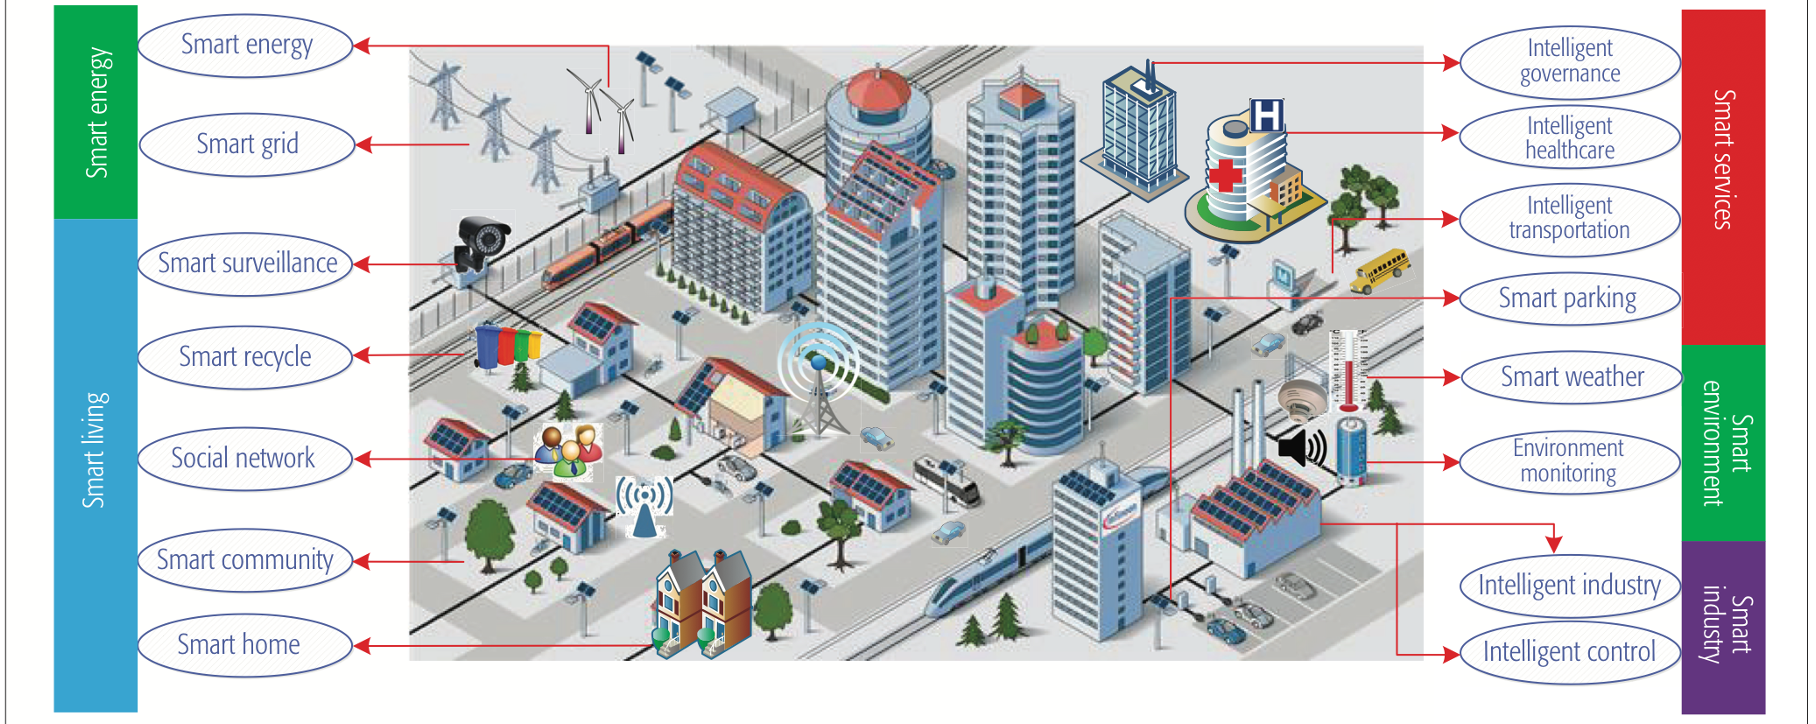
\includegraphics[width=\textwidth]{fundamentals/pictures/Smart_Applications}
    \caption{Darstellung der Teilsegmente einer Smart City zerlegt in ihre einzelnen Bestandteile \cite{Zhang2017}.}
    \label{fig:smart-applications}
\end{figure}

\noindent In den nächsten beiden Unterkapiteln werden basierend auf der Verwendung in der späteren Analyse die beiden Bereiche \textbf{Smart Home} und \textbf{Smart City} genauer definiert und eingeordnet.

\paragraph{Smart Home.}
\label{sec:Grundlagen:para:Smart Home}
Das \textbf{Smart Home} beschreibt als konkrete Einheit die Integration von \ac{iot} in die Behausungen eines Individuums. Durch die Verwendung von sogenannten \acl{wsn} haben die einzelnen Smart Devices innerhalb des Netzwerkes die Fähigkeit miteinander kommunizieren und Daten über ihren aktuellen Zustand auszutauschen \cite{Biljana2017}. Die hierbei eingesetzten Typen von Apparturen können beispielsweise dem kontextuellen Rahmen von \textbf{Sicherheit}, \textbf{Energie-Effizient \& Komfort} und \textbf{Gesundheit \& Wohlbefinden} zugeordnet werden. Fokus der Integration von \ac{iot} in den Wohnraum besteht in allgemeiner Verbesserung der Lebensqualität und Steigerung des Wohlbefinden \cite{Bastos2018}. Nachfolgend eine Auflistung von möglichen Gerätetypen innerhalb oben genannten Bereiche.

\begin{itemize}
	\item Sicherheit
		\begin{itemize}
			\item Intelligente Türschlösser
			\item Überwachungskameras
		\end{itemize}
	\item Energie-Effizienz \& Komfort
		\begin{itemize}
			\item Remote-steuerbare Lampen
			\item Intelligente Heizkörper
			\item Sensoren für den Energieverbrauch
		\end{itemize}
	\item Gesundheit und Wohlbefinden
		\begin{itemize}
			\item Sensor für Herzfrequenz
			\item Schrittzähler
		\end{itemize}
\end{itemize}

\paragraph{Smart City.}
\label{sec:Grundlagen:para:Smart City}
Als übergeordneter Kontext beschreibt die \textbf{Smart City} den Zusammenschluss mehrerer individueller \textbf{smarter Umgebungen}, auch \textbf{Smart Environments} genannt, die innerhalb dieses Konstruktes zusammengefasst werden können. Wie aus Abbildung \ref{fig:smart-applications} ersichtlich kann das bereits in \ref{sec:Grundlagen:para:Smart Home} beschriebene \textbf{Smart Home} als Bestandteil einer \textbf{Smart City} verstanden und somit auch als potentielle Datenquelle für die Nutzung durch diese übergeordnete Kontrollinstanz verwendet werden. Die hierdurch ermöglichten Synergien fördern Entwicklungspotentiale unter anderem in den Bereichen \textbf{öffentliche Dienste}, \textbf{Verkehrsmanagement}, \textbf{Energieverbrauch}, \textbf{Luftqualität \& Lärmbelastung} und die \textbf{Reduzierung von operationellen Kosten} \cite{Bastos2018}.
Im Rahmen der verwendeten Literatur, beispielsweise \cite{Bastos2018,Cui2018,SecPrivSmartCity2021}, lässt sich in die nachfolgenden kleineren Einheiten unterscheiden. Da sich die Definitionen dieser Konstrukte auf Basis der betrachteten Aspekte unterscheiden kann, erhebt diese Liste keinen Anspruch auf Vollständigkeit und gibt nur einen groben Überblick über die aktuelle Situation.

\begin{itemize}
	\item \textbf{Smart Energy}: Umfasst Themengebiete wie \textit{Smart Energy}, \textit{Smart Grid}, \textit{Smart Surveillance} und \textit{Smart Recycle}
	\item \textbf{Smart Services}: Beschreibt die Ressorts \textit{Intelligent Governance}, \textit{Intelligent Healthcare}, \textit{Intelligent Transportation} und \textit{Smart Parking}
	\item \textbf{Smart Living}: Enthält neben dem \textit{Social Network}, \textit{Smart Community} auch das bereits beschriebene \textit{Smart Home}
	\item \textbf{Smart Environment}: Adressiert die Gebiete \textit{Smart Weather} und \textit{Environment Monitoring}
	\item \textbf{Smart Industry}: Umschließt die Sachgebiete von \textit{Intelligent Industry}, auch häufig als Industrie 4.0 bezeichnet, und \textit{Intelligent Control}
\end{itemize}

\noindent Basierend auf den vorangegangenen Grundlagen werden nun aufbauend die Analyse der Datenschutzkonformität der \ac{iot}-Geräte innerhalb der Kontext \textbf{Smart Home} und \textbf{Smart City} durchgeführt.
